\chapter{La Gamification}
La gamification è l'utilizzo di elementi e meccaniche di gioco in contesti non ludici, come ad esempio l'istruzione, la salute, il lavoro o il marketing, al fine di aumentare l'impegno, la motivazione e la partecipazione degli utenti. Essa può essere applicata attraverso una varietà di tecnologie e utilizza principi di design e di psicologia del gioco, come le regole, le sfide, le ricompense, i feedback e le progressioni, per incentivare il comportamento desiderato e migliorare l'esperienza del partecipante.
L'obiettivo della gamification è quello di rendere le attività più interessanti, coinvolgenti e gratificanti, spingendo gli utenti a raggiungere obiettivi specifici e a perseguire comportamenti positivi.\\
\\
Un esempio del potenziale della gamification lo possiamo notare guardando alla famosa casa software Microsoft. Il gruppo di testing gestita da Ross Smith aveva l'incarico di trovare e correggere gli errori del software di Office. Il problema con ciò era l'enorme quantità di lavoro che dovevano svolgere per controllare ogni possibile scenario, ogni singola frase per ogni lingua il cui software era disponibile.\\
Ross Smith trovo una soluzione intelligente al problema. Coinvolse tutti i dipendenti microsoft di provenienti da tutto il mondo in un gioco che consisteva nel trovare errori di traduzione. Per ogni frase trovata venivano assegnati punti di cui ne sarebbero stati tenuti traccia su una classifica. Per assicurarsi che non venivano indicate frase casuali dai giocatori, introdusse anche diversi errori di traduzione di proposito e il gioco prendeva nota dei risultati delle persone, così poteva capire se una certa persona indicava errori dove non c'erano di proposito.
Dei 4500 dipendenti che hanno partecipato molti lo hanno descritto come un passatempo piacevole e a volte anche che dava dipendenza e durante il periodo di questo esperimento vennero corretti circa mezzo milione di errori di traduzione e trovati 6700 bugs.

\subsection{Considerazioni da fare}
Prima di procedere con il processo di gamificazione occorre fare alcune valutazioni per capire se la \textit{gamification} è adatta alla situazione cui ci si pone di fronte.
\begin{itemize}
  \item \textbf{Motivazione:} da dove si può trarre valore dall'incoraggiamento di un comportamento?\\
  La gamfication è una forma di design motivazionale. Si tratta fondamentalmente di un mezzo per convincere le persone a comportarsi in un certo modo. In generale, i clienti più motivati acquisteranno di più e i lavoratori più motivati otterranno prestazioni migliori.
È improbabile che un prodotto tragga un beneficio significativo dalla fidelizzazione, perché di solito gli acquirenti scelgono questo tipo di prodotti solo in base al prezzo. D'altro canto, un'azienda come Apple, i cui clienti sono già appassionati, potrebbe ritenere che le meccaniche di gioco distraggano dal prodotto stesso o generino attività che non producono entrate aggiuntive.\\
\\
Ci sono tre tipi principali di attività per le quali la motivazione è particolarmente importante: il lavoro creativo, i compiti banali e il cambiamento di comportamento. Alcuni compiti implicano legami emotivi, abilità uniche, creatività e lavoro di squadra.
Sono queste le attività ad alto valore aggiunto o le relazioni con i clienti che contribuiscono in misura maggiore al vantaggio competitivo. Sono anche ottimi candidati per la gamificazione. Che si tratti di progettare un nuovo prodotto o di coltivare ambasciatori di marca di alto livello, questi compiti dipendono fortemente dalla motivazione.
Le persone lavorano al meglio quando sono profondamente impegnate e concentrate, persino appassionate, su ciò che stanno facendo. La gamificazione può offrire loro un'esperienza soddisfacente, personalizzata e costantemente gratificante.\\
All'altra estremità dello spettro ci sono i compiti banali che implicano il rispetto di procedure definite e che sono di natura puramente individuale. Anche la gamificazione può essere efficace in queste situazioni, ma deve essere fatta in modo diverso. L'obiettivo non è ingannare le persone per far loro tollerare un lavoro noioso, ma aiutarle a trovare un senso in questa attività. Infine, ci sono gli scenari di cambiamento del comportamento, in cui le persone capiscono che qualcosa è buono per loro, ma hanno difficoltà a farlo.
La sfida consiste nel rendere l'attività abituale.
  \item \textbf{Scelte significative:} sono le attività sufficentemente interessanti?\\
  I giochi di successo richiedono l'autonomia dei giocatori, sia che si tratti di consumatori che decidono di acquistare, sia che si tratti di lavoratori che decidono di intraprendere azioni che vanno oltre le loro mansioni. I giocatori non possono limitarsi a seguire un percorso prestabilito. Quando si rendono conto che non c'è un motivo intrinseco per preoccuparsi, qualsiasi spinta all'impegno derivante dalle meccaniche di gioco viene meno.
Scelte significative significano semplicemente opzioni che danno al giocatore una certa libertà di scelta, e conseguenze evidenti che derivano da tali decisioni. Un sistema di gioco che offre ricompense ma non scelte diventerà rapidamente noioso per la maggior parte dei giocatori.
  \item \textbf{Struttura:} i comportamenti desiderati possono essere modellati tramite un algoritmo?\\
  I giochi scatenano la qualità non misurabile del divertimento, ma la gamificazione richiede algoritmi per misurare e rispondere alle azioni. Inoltre, deve essere facile registrare o tracciare le attività degli utenti, in modo che i dati rilevanti possano confluire nei sistemi online che gestiscono il gioco.
Il gigante dell'elettronica di consumo Samsung ha integrato il suo sito web con un programma chiamato Samsung Nation. I giocatori possono guadagnare badge e salire di livello recensendo prodotti, guardando video e fornendo risposte alle domande sui prodotti. Samsung ha creato un sistema di punti che assegna un valore a tutte queste azioni. La condivisione di un'azione su Twitter vale 100 punti, mentre la registrazione di un prodotto Samsung appena acquistato ne vale 500.
Il rapporto di 5 a 1 è arbitrario, ma rappresenta una stima approssimativa dei benefici relativi delle due attività per la rete. Molti sistemi di gestione non hanno bisogno di valori di punti specifici di questo tipo, ma tutti richiedono un modo per modellare le opzioni in modo algoritmico. Se non si dispone di un modo strutturato per valutare, ad esempio, la differenza tra un'innovazione proposta di alta qualità e una scadente, è probabile che \textit{gamification} non sia un buon mezzo per motivare i partecipanti.
  \item \textbf{Potenziali conflitti:} Riesce il gioco ad evitare conflitti con strutture motivazionali esistenti?\\
  Meccaniche di gioco, come le classifiche, possono demotivare i lavoratori quando sono collegate a ricompense tradizionali come stipendi e bonus. Quando vedono quanto sono in basso sul podio, molti lavoratori si arrendono.
La salita alla scala è troppo scoraggiante. Altri pensano che il lavoro è meno importante del gioco e lo tratteranno meno seriamente. Allo stesso modo, se la vostra promessa ai clienti è quella di far risparmiare loro tempo e aiutarli a diventare più efficienti, un'offerta che li incoraggia a perdere tempo in un'attività apparentemente frivola è una contraddizione.
È importante identificare tutti i modi esistenti per motivare la popolazione obiettivo e pensare a come potrebbero funzionare insieme alla gamificazione. È importante mettersi nei panni di un giocatore e chiedersi quale messaggio sta inviando la vostra organizzazione.
\end{itemize}

\section{Tipi di Gamification}
Abbiamo quindi visto i risultati di un esempio di gamification. A seconda di chi fa uso di questa tecnica e dell'obbiettivo possiamo individuare tre diversi tipi di Gamification.
\begin{figure}[h!]
  \centerline{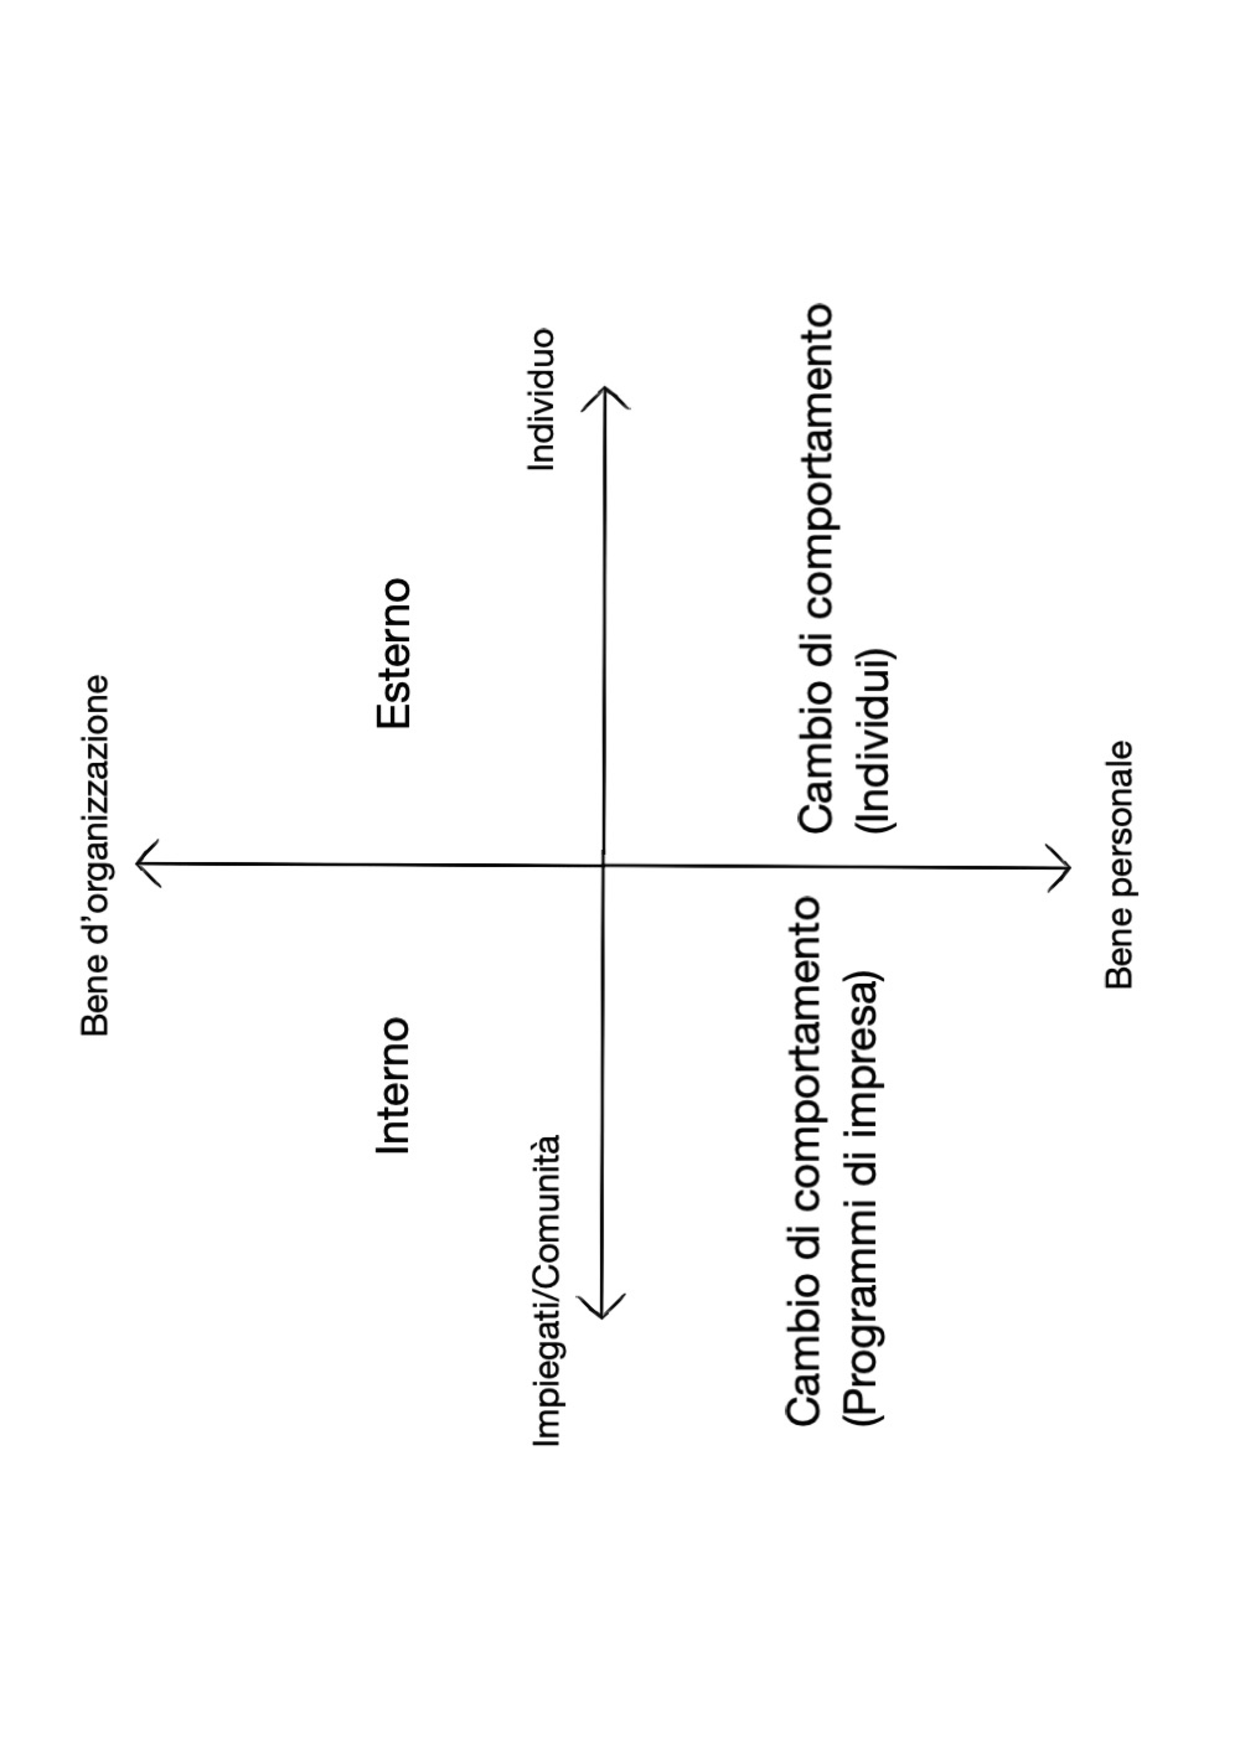
\includegraphics[height = 9 cm, width= 6 cm, angle=270]{figures/assi.pdf}}
  \caption{Piramide di Bloom}
\end{figure}
\subsection{Gamification interna}
Questo tipo di \textit{gamification} ha come scopo il miglioramento della produttività, promuovere innovazioni e in generale produrre risultati positivi per una organizzazione. Le persone che partecipano si conoscono già poichè fanno parte tutte dello stesso ambiente. Non è detto che condividano interessi comuni ma interagiscono regolarmente tra di loro e hanno lo stesso desiderio di essere riconosciuti all'interno dell'organizzazione cui fanno parte. La storia raccontata prima era un esempio di gamification interna.
\subsection{Gamification esterna}
Questo tipo di \textit{gamification} ha come partecipanti non più i dipendenti di una azienda ma i loro clienti. Gli obbiettivi in genere riguardano obbiettivi di mercato e mirano al miglioramento o ampliamento delle relazioni con i propri clienti con lo scopo che inizino o continuino ad usare il prodotto dell'azienda. Questa modalità è quella tipica dei giochi o videogiochi. Un esempio di questo tipo di \textit{gamification} lo troviamo guardando a \textit{Record Searchlight} un quotidiano americano. Quando c'è stato il passaggio dall'analogico al digitale nel campo dei giornali quotidiani \textit{Record Searchlight} rilevò che il loro profitto si stava assottigliando perché i clienti iniziarono a cercare le notizie online piuttosto che comprare le loro edizioni. Per combattere questa moda decisero di introdurre un sistema di medaglie. L'idea di fondo era quella di riconoscere agli utenti online diverse medaglie, ovvero immagini che apparivano affianco al loro nome, per chi lasciava commenti utili sugli articoli pubblicati. In tre mesi grazie a questa soluzione rilevò un incremento del 10\% del numero di commenti ricevuti e il tempo medio degli utenti sul sito è incrementato del 25\%.
\subsection{Gamfication di cambio di comportamento}
Infine la terza tipologia di \textit{gamification} mira a sviluppare nuove abitudini in una popolazione. Solitamente queste nuove abitudini promuovono uno stila di vita migliore o un cambiamento per il bene della comunità. Di questo tipo ci sono molti esempi da fare. Penso che tutti noi, ad un certo punto, abbiamo assistito o preso parte a qualche lezione sul codice stradale a bambini sotto forma di giochi organizzata da qualche scuola. In Svezia sono stati installati cartelloni che tossiscono se rilevano qualcuno che fuma nelle loro vicinanze. Sempre in Svezia sono stati installati cestini che quando vengono buttati rifiuti sembra che il rifiuto cada per metri e metri per terminare la loro caduto con un soddisfacente BONG.
\section{La Struttura PBL}

Andiamo a vedere la struttura più diffusa e semplice tra i sistemi \textit{gamificati} ovvero quella PBL (Points, badge, leadernboard). Con questa organizzazione si possono accumulare punti intraprendendo delle sfide e possono essere riscattati per ottenere dei premi. Tutti i punteggi dei vari giocatori vengono mostrati in una classifica per poter essere confrontati con quello degli altri. Ogni giocatore ha la possibilità di ottenere badge per i risultati ottenuti sulla piattaforma. \\
\\
I punti vengono utilizzati per incoraggiare le persone a fare qualcosa raccogliendoli.
L'ipotesi è che le persone comprino più widget o lavorino di più in cambio di punti.
È un approccio semplice che funziona per motivare le persone che amano collezionare o competere con gli altri.
\\
Ma i punti possono essere utilizzati in molti altri modi nella gamificazione:
\begin{itemize}
\item I punti tengono conto in modo efficace del punteggio, è il modo tipico in cui vengono utilizzati nei sistemi di gioco. I punti dicono al giocatore quanto sta facendo bene. Chi ha guadagnato 30'000 punti gioca da più tempo o con più successo di chi ha 18'000 punti. I punti possono anche delimitare i livelli. Ad esempio, "Hai bisogno di 10'000 punti per raggiungere il livello 5, a quel punto sblocchi il risultato 'super giocatore' e ottieni l'accesso a nuovi contenuti". In questo caso, i punti rappresentano il vero "spazio di gioco" di un gioco, perché ne definiscono l'avanzamento dall'inizio del gioco agli obiettivi.
\item I punti possono determinare lo stato di vittoria di un processo di gioco, ammesso che ne abbia uno. A volte si vogliono usare i punti per creare una condizione di vittoria: ad esempio, se si vuole mettere in palio un premio.
\item I punti creano un collegamento tra la progressione nel gioco e le ricompense estrinseche. Molti sistemi di gioco prevedono alcuni premi in denaro per il raggiungimento di determinati livelli o per il riscatto di punti virtuali: Con 1.000 punti si ottiene un set di coltelli da bistecca.
\item I punti forniscono un feedback. Un feedback esplicito e frequente è un elemento chiave nella maggior parte dei giochi di qualità, e i punti forniscono un feedback rapido e semplice. I punti sono tra i meccanismi di feedback più granulari. Ogni punto fornisce all'utente un piccolo feedback, dicendogli che sta facendo bene e che sta progredendo nel gioco.
\item I punti possono essere una visualizzazione esterna dei progressi. In un gioco multigiocatore, o in un ambiente in cui i membri della comunità o del posto di lavoro possono vedere i punteggi degli altri, i punti mostrano agli altri come si sta procedendo. Possono essere significativi come indicatore di status
\item I punti forniscono dati al progettista del gioco. I punti che gli utenti guadagnano possono essere facilmente tracciati e memorizzati. Permettono al progettista di analizzare importanti metriche sul sistema. Ad esempio, a che velocità gli utenti avanzano nel contenuto?
Sembra che stiano cadendo o si stiano bloccando in alcuni punti?
\end{itemize}
Tenete presente che i punti sono molto limitati. Sono uniformi, astratti, intercambiabili. In altre parole, un punto è un punto. Ogni punto in più indica semplicemente una grandezza maggiore, e niente di più. È uno dei motivi per cui i distintivi si trovano sempre in combinazione con i sistemi a punti.\\
\\
I badge sono una versione più grossa dei punti. Un badge è una rappresentazione visiva di un risultato ottenuto all'interno del processo di gamificazione. Alcuni badge indicano semplicemente un certo livello di punti. Fitbit è un sistema di gamizzazione che consente alle persone di utilizzare un contapassi wireless per tenere traccia del numero di chilometri percorsi a piedi o di corsa. Il sistema visualizza un badge quando l'utente supera determinate soglie di punti, come 50 miglia in una settimana o 10.000 passi in un giorno.
Altri badge indicano diversi tipi di attività.
Un sistema di badge ben progettato ha le seguenti caratteristiche motivazionali:
\begin{itemize}
\item I badge possono fornire agli utenti un obiettivo verso cui tendere, il che ha dimostrato di avere effetti positivi sulla motivazione.
\item I badge forniscono una guida su ciò che è possibile fare all'interno del sistema e generano una sorta di stenografia di ciò che il sistema dovrebbe fare.
È una caratteristica importante per far sì che l'utente si impegni con il sistema.
\item I badge sono un segnale di ciò che interessa all'utente e di ciò che ha fatto.
Sono una sorta di indicatore visivo della reputazione di un utente e gli utenti acquisiscono badge per cercare di mostrare agli altri ciò che sono in grado di fare.
\item I badge funzionano come status symbol virtuali e come rappresentazioni del percorso personale dell'utente attraverso il sistema di gamificazione.
\item I badge funzionano come marcatori tribali. Un utente che possiede alcuni degli stessi badge di altri utenti sentirà un senso di identità con quel gruppo e un design intelligente della gamificazione può collegare i badge a un sistema di identificazione del gruppo.
Uno degli attributi più importanti dei badge è il fatto che possono essere esibiti. Molti tipi diversi di badge possono essere assegnati per molti tipi diversi di attività, e la gamma di badge è limitata solo dall'immaginazione del progettista di gamificazione e dalle esigenze dell'azienda.
Questo permette al servizio di gamizzazione di coinvolgere più di un gruppo di utenti e di fare appello ai loro interessi in modi che un singolo sistema di punti non può fare.\\
\\
I badge possono avere una funzione di accreditamento. Uno degli aspetti positivi dei badge come credenziali è che sono assolutamente esauribili. Si può ricevere un badge per qualsiasi cosa, dalle sciocchezze alle cose serie. Alcune organizzazioni guardano addirittura ai badge come base per nuove forme di istruzione e formazione online. Non è così assurdo come potrebbe sembrare. Un diploma di un'università d'élite è una sorta di distintivo che promette un certo livello di abilità e di risultati da parte del titolare del diploma.\\
\\
Le classifiche sono l'ultima tappa della triade PBL, e forse la più problematica. Da un lato, i giocatori vogliono sapere dove si trovano rispetto ai loro compagni. Una classifica dà un contesto alla progressione come i punti o i badge non possono fare. Se le prestazioni nel gioco sono importanti, la classifica le rende pubbliche a tutti. Nella giusta situazione, le classifiche possono essere dei potenti motivatori. Sapere che bastano pochi punti in più per scalare una posizione o addirittura per emergere al primo posto può essere una forte spinta per gli utenti.\\
\\
D'altro canto, le classifiche possono essere fortemente demotivanti. Se si vede esattamente quanto si è indietro rispetto ai migliori giocatori, si può essere indotti ad abbandonare il gioco e a smettere di provarci. Le classifiche possono anche ridurre la ricchezza di un gioco a una lotta a somma zero per la supremazia, che intrinsecamente allontana alcune persone e fa sì che altre si comportino in modi meno desiderabili.\\
Ci sono vari modi per far funzionare le classifiche in un sistema di gioco. Una classifica non deve essere necessariamente un tabellone statico e non deve tenere conto di un solo attributo. In gamificazione, le classifiche possono tenere conto di una o più caratteristiche che il progettista vuole enfatizzare.
Non c'è nulla di male se più classifiche misurano cose diverse o se le classifiche non sono universali per tutti i partecipanti. Le classifiche possono anche essere collegate ai social network per fornire informazioni più contestuali, e meno preoccupanti sull'andamento dei giocatori.





\section{Elementi di un sistema di \textit{gamification}}
Ci sono tre categorie di elementi di gioco che sono rilevanti per la progettazione, elencati in ordine decrescente di astrazione questi sono: la dinamica, la meccanica e i componenti. Ogni meccanica è legata a una o più dinamiche e ogni componente è legato a uno o più elementi di livello superiore.
\subsection{Dinamiche}
  Le dinamiche di gioco più importanti:
  \begin{itemize}
    \item Vincoli (limitazioni o scambi forzati)
    \item Emozioni (curiosità, competitività, frustrazione, felicità)
    \item Narrazione (una trama coerente e continua)
    \item Progressione (crescita e sviluppo del giocatore)
    \item Relazioni (interazioni sociali che generano sentimenti di cameratismo, status, altruismo)
  \end{itemize}
  Le dinamiche sono gli aspetti generali del sistema di gioco da considerare e gestire, ma che non si possono mai inserire direttamente nel gioco. Nel mondo del management, le analogie sono lo sviluppo dei dipendenti e la creazione di una cultura dell'innovazione. I leader e manager aziendali raramente, se non mai, hanno l'opportunità di progettare un'azienda da zero. Piuttosto, devono spingere un'organizzazione già esistente nella giusta direzione attraverso assunzioni e promozioni, pratiche di gestione e così via. Quando si crea un sistema di gestione, invece, si può fare quello che si vuole. Pensare fuori dagli schemi nella gamificazione è il modo migliore di agire.
  \subsection{Meccaniche}
  Le meccaniche sono i processi di base che portano avanti l'azione e generano il coinvolgimento del giocatore. Possiamo identificare dieci importanti meccaniche di gioco:
  \begin{itemize}
\item Sfide (enigmi o altri compiti che richiedono una certa abilità per essere risolti)
\item Chance (elementi di casualità)
\item Competizione (un giocatore o un gruppo vince e l'altro perde)
\item Cooperazione (i giocatori devono lavorare insieme per raggiungere un obiettivo condiviso)
\item Feedback (informazioni sull'andamento del giocatore)
\item Acquisizione di risorse (ottenere oggetti utili o collezionabili)
\item Ricompense (benefici per qualche azione o risultato)
\item Transazioni (scambi tra giocatori, direttamente o tramite intermediari)
\item Turni (partecipazione sequenziale di giocatori alternati)
\item Stati di vittoria (obiettivi che fanno di un giocatore o di un gruppo il vincitore; gli stati di pareggio e di
  perdita sono concetti correlati).
\end{itemize}
Ogni meccanica è un modo per realizzare una o più delle dinamiche descritte. Un evento casuale, come un premio che appare senza preavviso, può stimolare il senso di divertimento e la curiosità dei giocatori. Può anche essere un modo per coinvolgere i nuovi partecipanti o per mantenere i giocatori più esperti.
\subsection{Componenti}
I componenti sono forme più specifiche che la meccanica o la dinamica possono assumere.
Quelli più importanti sono:
\begin{itemize}
\item Obiettivi (obiettivi definiti)
\item Avatar (rappresentazioni visive del personaggio del giocatore)
\item Badge (rappresentazioni visive dei risultati ottenuti)
\item Combattimenti con i boss (sfide particolarmente difficili al culmine di un livello).
di un livello)
\item Collezioni (serie di oggetti o distintivi da accumulare)
\item Combattimento (una battaglia definita, in genere di breve durata)
\item Sblocco di contenuti (aspetti disponibili solo quando i giocatori raggiungono gli obiettivi)
\item Regali (opportunità di condividere le risorse con gli altri)
\item Classifiche (visualizzazioni dei progressi e dei risultati ottenuti dai giocatori)
\item Livelli (fasi definite della progressione del giocatore)
\item Punti (rappresentazioni numeriche della progressione del gioco)
\item Missioni (sfide predefinite con obiettivi e ricompense)
\item Grafici sociali (rappresentazione della rete sociale dei giocatori all'interno del gioco)
\item Squadre (gruppi definiti di giocatori che lavorano insieme per un obiettivo comune)
\end{itemize}
Come ogni meccanica è legata a una o più dinamiche, ogni componente è legata a uno o più elementi di livello superiore.

\section{Processo di \textit{gamification}}

Con i concetti essenziali di gioco che abbiamo definito ora possiamo entrare nella fase di design del nostro sistema gamificato.
L'implementazione migliore è quella in cinque fasi:
\begin{itemize}
\item \textbf{DEFINIRE} gli obiettivi aziendali
\item \textbf{DELINEARE} i comportamenti target
\item \textbf{DESCRIVERE} gli attori
\item \textbf{DISEGNARE} i cicli di attività
\item \textbf{NON DIMENTICARE} IL DIVERTIMENTO!
\end{itemize}
\subsection{Definire gli obbiettivi aziendali}

Per una gestione efficace, è fondamentale avere una comprensione ben sviluppata dei propri obiettivi.
Questi sono obiettivi specifici di performance del vostro sistema di gestione, come l'aumento della fidelizzazione dei clienti, la costruzione della fedeltà al marchio o il miglioramento della produttività dei dipendenti. Se non si inizia con questa fase, il progetto di gamificazione può essere avviato, ma probabilmente alla fine fallirà. Una gestione efficace a volte può produrre risultati che non sono necessariamente utili. Per evitare questa trappola, il primo passo consiste nel fare un elenco di tutti i potenziali obiettivi. Ogni obiettivo deve essere il più preciso possibile, l'elenco iniziale può essere ampio a piacere perché probabilmente in seguito verrà ridotto. Forse si vuole attirare gli studenti delle scuole superiori delle comunità a basso reddito a utilizzare il proprio strumento educativo di finanza personale, o forse si vuole che i propri dipendenti suggeriscano idee fuori dagli schemi per nuove opportunità commerciali. Bisogna classificare questo elenco in termini di importanza. Potrebbe essere necessario scambiare obiettivi minori con altri più significativi. A questo punto, scorrete l'elenco e depennate tutto ciò che è un mezzo piuttosto che un fine. In altre parole far accumulare punti e badge agli utenti non è un motivo per implementare un sistema di gioco, ma è qualcosa che avviene all'interno di un sistema. Avere un gran numero di giocatori che visitano il vostro sito web è un fine solo se ha un valore diretto per voi, altrimenti potrebbe generare costi di supporto senza entrate concomitanti. Infine spiegate per ogni obbiettivo come può essere vantaggioso per la vostra organizzazione. La lista è uno strumento per mantere la concentrazione sulle priorità durante la progettazione e lo sviluppo, anche se si ci sono stati dei cambiamenti di priorità.

\subsection{Delineare i comportamenti desiderati}

Una volta individuato il motivo della gamification, è necessario concentrarsi su ciò che si vuole far fare ai giocatori e su come misurarlo. Comportamenti e metriche sono meglio considerati insieme. I comportamenti desiderati devono essere concreti e specifici, ad esempio:
\begin{itemize}
\item Lasciare una recensione del prodotto.
\item Rivisitare un parco divertimenti per la seconda volta nell'anno.
\item Andare in palestra per un'ora alla settimana.
\item Condividere le esperienze agli amici tramite Facebook.
\item Presentare gli amici come nuovi clienti alla propria banca.
\item Visitare il proprio ristorante.
\end{itemize}
I comportamenti ricercati devono promuovere gli obiettivi aziendali finali precedentemente definiti, anche se la relazione può essere indiretta. Ad esempio, far sì che gli utenti trascorrano più tempo sul proprio sito o che parlino dei vostri prodotti su Facebook non si traduce immediatamente in un guadagno, ma può comunque essere auspicabile. Occorre individuare il maggior numero possibile di comportamenti. Per dare agli utenti una vasta scelta di opzioni e attività da perseguire in base alle loro preferenze.
Una volta elencati tutti i comportamenti desiderati, occorre definire le metriche di successo. Queste sono i modi in cui si traducono i comportamenti in risultati quantificabili, che possono essere più o meno trasparenti al giocatore. I punti possono essere una di queste metriche e non occorre necessariamente che siano visibili al giocatore, servono al sistema per generare il feedback delle azioni che i giocatori effettuano.
Gli "stati di vittoria" costituiscono un secondo tipo di metrica di successo. Ma bisogna prestare attenzione nell'usarli in quanto implicano la possibilità di perdere e per alcuni potrebbe essere demoralizzante per chi partecipa. È importante ricordare che l'obbiettivo della gamificazione è motivare l'utente per fargli raggiungere determinati obbiettivi organizzativi. È possibile aggirare in qualche modo queste limitazioni creando stati di vittoria localizzati o temporali.
Si potrebbe rendere i badge progressivi, dove non più sei in possesso del badge oppure no ma che hai il badge è di grado 3 su 5, incoraggiando così una progressione continua.

\subsection{Descrivere gli attori}

Dobbiamo ora farci un'idea di chi utilizzerà il sistema, come possiamo motivarli?
Bisogna capire cosa potrebbe demotivare i giocatori. Un motivo potrebbe essere la mancanza di volontà, che si può risolvere con un approccio orientato all'impegno, oppure per mancanza di capacità, risolvibile tramite sistemi di progressione che accompagnino dolcemente il giocatore lungo la curva di difficoltà. È opportuno segmentare i giocatori in modo che il sistema sia adatto a più di un sottogruppo. La segmentazione è una pratica comune nel marketing e nelle risorse umane. In questo caso è ancora più importante. Poiché i giochi e i sistemi di gioco offrono tipicamente delle scelte ai giocatori, non è necessario scegliere un unico segmento a cui rivolgersi.
I progettisti di giochi hanno diversi modelli di tipologie di giocatori che utilizzano come punti di partenza per la segmentazione.
Il più noto è stato inventato alla fine degli anni '80 dal ricercatore di giochi Richard Bartle, che stava studiando i primi giochi online multiplayer basati su testo.
Bartle ha distinto quattro tipi di giocatori: realizzatori, esploratori, socializzatori e assassini. I giocatori realizzatori amano l'emozione di salire di livello o di guadagnare un distintivo; gli esploratori vogliono scoprire nuovi contenuti; i socializzatori vogliono impegnarsi con gli amici; e gli assassini vogliono imporre la loro volontà sugli altri, in genere sconfiggendoli.
I migliori giochi e sistemi di gioco hanno qualcosa per ogni categoria e la modellazione dei giocatori è un modo per definire la segmentazione e guidare ulteriormente il processo di progettazione.
Questo processo possiamo svilupparlo dividendo gli utenti in vari gruppi in base al loro comportamento. Per ogni gruppo associamo un volto, un nome e una storia che accomuna tutti quelli che fanno parte di quel gruppo.
Ora domandiamoci Dove si collocano tra i tipi di giocatori Bartle? Quali sono le loro speranze e le loro paure? I loro talenti? I loro hobby? Più dettagliata è la descrizione di queste "persona" meglio è. Se le "persona" non sono veritiere, se non rispecchiano il vostro probabile pubblico, bisogna cambiarli finché non lo sono. Questi modelli di personaggi saranno alla base delle vostre attività di progettazione. Tutto questo serve per "conoscere" l'utente per poter immaginarsi meglio come esso risponderà alle varie meccaniche del sistema. L'ultima dimensione da considerare è il ciclo di vita del giocatore. Tutti iniziano come novizi e in quanto tali hanno bisogno di essere seguiti per imparare le regole. Potrebbero aver bisogno di una mano per avere successo. Una volta che il novizio diventa abituale, ha bisogno di novità per rimanere fedele all'attività. Ciò che all'inizio era nuovo e stimolante ora è inutile. Infine, il giocatore diventa un esperto. Gli esperti hanno bisogno di sfide abbastanza difficili da tenerli impegnati. tendono anche a volere un rinforzo esplicito del loro
status. Non tutti i giocatori si troveranno nella stessa fase allo stesso tempo, anche se più a lungo il sistema funziona, più si orienterà verso la parte più esperta. È necessario offrire opportunità ai giocatori in tutte le fasi.

\subsection{Disegnare i cicli di attività}

I giochi tipicamente hanno un inizio e una fine, ma non è detto che il percorso che collega i due sia sempre lineare. Il modo più utile per modellare l'azione in un sistema di gamificazione è attraverso i cicli di attività. Ci sono due tipi di cicli da sviluppare: i cicli di coinvolgimento e le scale di progressione. I cicli di coinvolgimento descrivono, a livello generale, cosa fanno i giocatori, perché lo fanno e cosa fa il sistema in risposta. Le scale di progressione forniscono una prospettiva macro sul comportamento del giocatore.\\
\\
In un circuito di coinvolgimento le azioni del giocatore derivano dalla motivazione e a loro volta producono un feedback sotto forma di risposte da parte del sistema, come l'assegnazione di punti.
Quel feedback motiva l'utente a compiere ulteriori azioni, e così via.
L'elemento chiave è il feedback. Esso è parte di ciò che rende i giochi così efficaci come motivatori.
Le azioni producono immediatamente risposte visibili. L'utente vede immediatamente la sua posizione e quando fa qualcosa di buono lo sa sempre. Il feedback è ciò che crea la motivazione per ulteriori azioni.
Questo ciclo di coinvolgimento è il processo di base del vostro sistema di gestione. Tuttavia, non coglie i modi in cui i giocatori avanzano. Se l'esperienza è esattamente la stessa al giorno 100 come al giorno 1, la maggior parte dei giocatori si annoia. È qui che entrano in gioco le scale di progressione.\\
\\
Le scale di progressione indicano che l'esperienza di gioco cambia man mano che i giocatori la attraversano.
di solito significa un livello crescente di sfide. Ogni prima scala, chiamata \textit{”onboarding"}, deve essere così semplice e guidata da attirare i giocatori nel gioco. Una volta che il giocatore ha superato questo ostacolo, la difficoltà dovrebbe idealmente aumentare a tassi variabili, lungo quelle che vengono chiamate curve di interesse. Il modello utilizzato nella maggior parte dei giochi prevede un aumento costante della difficoltà, seguito da un periodo di relativa facilità e da una sfida importante alla fine di ogni segmento. Il periodo di riposo permette ai giocatori di riprendere fiato. Permette inoltre di provare la soddisfazione della padronanza: la sensazione di essere diventati esperti in qualche parte del gioco.
La sfida finale di un livello offre una diversa esperienza di padronanza. Le sfide più grandi, che i giocatori riescono a superare a malapena, sono quelle che producono l'esplosione di emozioni positive.
Non è da trascurare l'incorporamento di una certa dose di casualità. Alle persone piacciono le sorprese. Il nostro cervello preferisce una piccola possibilità casuale di ottenere una grande ricompensa alla certezza di una ricompensa modesta che, nel corso del tempo, raggiunge una media più alta.
Basta guardare la popolarità delle slot machine per convincersi di questa affermazione.
 Le sorprese, anche quelle piccole e positive, sono il modo per sfuggire a quello che viene definito il treadmill edonico: la tendenza a dare per scontato ogni progresso e a chiedere ricompense sempre più grandi per evitare la noia.

\subsection{Non dimenticare il divertimento}

L'ultima cosa da fare prima di iniziare a implementare un sistema di gamificato è fare un passo indietro e porsi una semplice domanda: È divertente?
Un progetto di gamificazione fatto bene è una cosa seria. Tuttavia, il divertimento non dovrebbe mai trascurato. Se gli utenti percepiscono il sistema di gamificato come divertente, è probabile che tornino. È opportuno valutare costantemente l'aspetto estetico del sistema e considerare se è divertente da giocare.
Possiamo porci le domande: I giocatori parteciperebbero volontariamente al vostro sistema? Se non ci fossero ricompense estrinseche, sarebbero comunque propensi a giocare? Se la risposta è no, allora dovreste pensare a cosa potrebbe rendere il vostro sistema più divertente. Il divertimento ha molte dimensioni e non bisogna dare per scontato che tutti vogliano lo stesso tipo di divertimento. Nicole Lazzaro, game designer e consulente esperta degli aspetti emotivi dei giochi, ha trovato quattro tipi distinti di divertimento studiando un gruppo di giocatori.
\begin{itemize}
  \item Il "divertimento difficile" è una sfida o un rompicapo che diverte per il piacere di superarlo.
  \item Il "divertimento facile" è un divertimento occasionale, un modo per sfogarsi senza impegnarsi troppo.
  \item  "Stati alterati", è il divertimento sperimentale. È il piacere di provare nuovi personaggi e nuove esperienze.
  \item  "fattore persone" è essenzialmente il divertimento sociale: il tipo di divertimento che dipende dall'interazione con gli altri, anche se competitiva.
\end{itemize}
